\newcommand{\figureElectronicsWaterVessels}[1]{
  \def\lang{\detokenize{#1}}
  \def\langRu{\detokenize{ru}}
  \def\langEn{\detokenize{en}}
  \def\figureCaption{XXX: No translation.}
  \def\figureVesselA{XXX: No translation.}
  \def\figureVesselB{XXX: No translation.}
  \ifx \lang\langRu
  \def\figureCaption{
    Пример двух ёмкостей: с водой (А) и пустая (Б).
  }
  \def\figureVesselA{А}
  \def\figureVesselB{Б}
  \fi
  \ifx \lang\langEn
  \def\figureCaption{
    An example of two vessels: one filled with water (A) and one that is
    empty (B).
  }
  \def\figureVesselA{A}
  \def\figureVesselB{B}
  \fi
  \begin{figure}[ht]
    \centering
    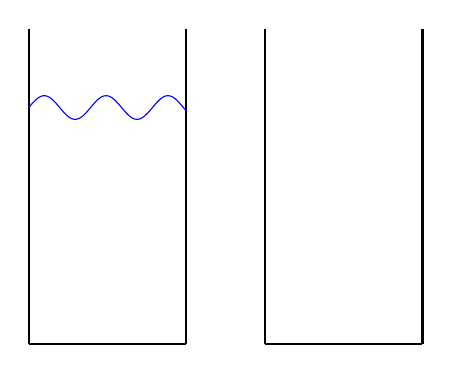
\begin{tikzpicture}[
        declare function={f1(\x) = 0.15 * sin(8.0 * deg(\x));
      }]

      \draw[thick] (0, 0) -- (0, 4);
      \draw[thick] (2, 0) -- (2, 4);
      \draw[thick] (0, 0) -- (2, 0);

      \draw[thick] (3, 0) -- (3, 4);
      \draw[thick] (5, 0) -- (5, 4);
      \draw[thick] (3, 0) -- (5, 0);

      \begin{scope}[yshift=3cm, color=blue]
        \draw (0, 0) plot[
          domain=0:2, variable=\x, samples=200, smooth
        ] ({\x}, {f1(\x)});
      \end{scope}

      \draw (1, 0) node[below] {\figureVesselA};
      \draw (4, 0) node[below] {\figureVesselB};

    \end{tikzpicture}
    \caption{\figureCaption}
    \label{fig:electronics-circuits-0}
  \end{figure}
}
